
\newcommand{\dpt}[1]{\frac{\partial #1}{\partial t}}

\subsubsection{Advection of a generic conserved quantity}

Consider the advection of a generic {\em conserved} quantity $\phi$ by a continuous velocity field
\be
\dert \phi + \nabla \cdot ( \phi \U)  = 0. \label{phiconv}
\nd
We assume that $\phi$ is smoothly varying except on the interface where it may be discontinuous.
Indeed finding a correct scheme for the advection of this discontinuity, at the same speed as the advection of the 
volume fraction, is the goal of the present study.
The smoothness of the advected quantity away from the interface
is verified for the density $\rho$, the momentum $\rho \U$ or the internal energy 
$\rho e$. 
\newcommand\pijk{\phi_{i,j,k}}
Integrating the advection equation in time one obtains
\be
{\pijk^{n+1} - \pijk^{n}} = - \sum_{\rm{faces}\, f} F^{(\phi)}_f, \label{sumfp}
\nd
where the sum of the right-hand side is the sum over faces $f$ of cell $i,j,k$ 
of the fluxes $F^{(\phi)}_f$ of $\phi$. In equations, $F_f^{(\phi)}$ is defined in a similar manner to 
equation (\ref{faceint}) for the color function fluxes. 
\be
F_f^{(\phi)} = \int_{t_n}^{t_{n+1}} {\rm d}t \int_{f} u_f(\X,t) \phi(\X,t)  {\rm d}\X, \label{pfaceint}
\nd
where 
\be
u_f = \U\cdot \N_f, \label{uf}
\nd
 and $\N_f$ is the unit normal vector of face $f$, pointing outwards of cell $i,j,k$. 
In order to ``extract'' the discontinuity the flux can be expressed as
\be
F_f^{(\phi)} = 
\int_{t_n}^{t_{n+1}} {\rm d}t \int_{f} [ u_f  H \phi  +  u_f (1-H) \phi ]  {\rm d}\X , \label{fluxphi}
\nd
which can be re-expressed in terms of the fluxes $F^{(c)}$ in eq. (\ref{faceint}) as
\be
F_f^{(\phi)} = 
\bar \phi_1 \int_{t_n}^{t_{n+1}} {\rm d}t \int_{f} u_f H   {\rm d}\X + \bar \phi_2 \int_{t_n}^{t_{n+1}} {\rm d}t \int_{f}   
u_f (1-H) {\rm d}\X \label{barphi}
\nd
where 
\be 
\bar \phi_s = \frac{\int_{t_n}^{t_{n+1}} {\rm d}t \int_{f}  u_f  H_s \phi \, {\rm d}\X}{\int_{t_n}^{t_{n+1}} {\rm d}t \int_{f}  
u_f  H_s\,{\rm d}\X},  \label{barphi2}
\nd
and $H_1=H$, $H_2= 1-H$. This can be expressed as  
\be
F_f^{(\phi)} = \bar \phi_1 F_f^{(c)} +  \bar \phi_2 F_f^{(1-c)},
\nd
where $F_f^{(c)}$ is the flux of $H$ defined in (\ref{faceint}) and  $F_f^{(1-c)}$ is the flux 
obtained by replacing $H$ by $1-H$ in  (\ref{faceint}). 

\subsubsection{Cloning the tracers}

When a cell is cut by the interface, and the field $\phi$ is non-smooth, it becomes difficult to estimate
the integrals in (\ref{barphi}). A possibility is to define two new fields $\phi_{1,2}$ so that 
$\phi_s = \phi$ inside phase $s$. Then
\be
\phi = H \phi_1 + (1-H)\phi_2.
\nd
In the discretized equation, two discrete fields $\phi_{s,i,j,k}$ are defined over the entire domain $\Omega$.
This is more costly in memory usage but simplifies considerably the computation of the averages in Equation
 (\ref{barphi}). The two equations (\ref{phiconv}) and (\ref{interfadv}) are now replaced by three equations,
the same volume fraction equation  (\ref{interfadv}) and the two equations
\bea
\dert \phi_1 + \nabla \cdot ( \phi_1 \U)  &= 0&  \label{pcv1}, \\ 
\dert \phi_2 + \nabla \cdot ( \phi_2 \U)  &= 0& \label{pcv2} . 
\nda
The three equations (\ref{interfadv},\ref{pcv1}-\ref{pcv2}) now imply (\ref{phiconv}). This addition of a pair of ``cloned'' variables to help deal with large variations of density is similar to the methods used for the resolution of the momentum and energy equations for compressible flow. For example Saurel and Abgrall used two density, momentum and energy variables in ref. \cite{Saurel99}, leading to their seven-equations model, while Allaire, Clerc and Kokh use two density variables in \cite{allaire02}, leading to their five-equations model. The addition of a cloned tracer variable in incompressible isothermal flow was also implemented by Popinet in the ``Basilisk'' code \cite{basilisk}. 

\subsubsection{Advection of the density field}

Let us now apply the above considerations to the advection of the density
field by a general continuous velocity field.
Although in the incompressible case the density follows trivially the color
function, it will allow us to introduce an important point
about the equivalence of tracer and VOF advection. 
The density $\rho(\X,t)$ obeys eq. (\ref{phiconv}) with 
$\phi = \rho$. %There is no compression term in eq. (\ref{phiconv}). 
The advection of density may be made consistent with the advection of the color function by 
using fluxes  $F_f^{(c)}$ and estimating
the average occuring in equation (\ref{barphi2}),  
$\bar \phi_1 = \bar \rho$ from averages over control volumes or approximations on faces.

The case relevant here is that of an incompressible velocity field, with uniform density in each phase. 
Then $\rho$ is exactly proportional to $H$ (Eq. \ref{muH}).
The constancy of $\rho$ allows to extract it trivially from the integrals in eq. (\ref{barphi}) 
and to obtain {\em exactly} $\bar \rho_s = \rho_s$. 
Then the flux of $\rho$ is  
\be
F_f^{(\rho)} = \rho_1 F_f^{(c)} +  \rho_2 F_f^{(1-c)}.\label{fluxrho}
\nd
Using this flux definition for $\rho$, and any VOF method for the fluxes of the color function, 
one obtains a conservative method for $\rho$ since eq. (\ref{sumfp}) 
evolves $\rho$ as a difference of fluxes. 
That is, one conserves the total mass and 
$\sum_{i,j,k} \rho^{(n)}_{i,j,k} =  \sum_{i,j,k} \rho^{(n+1)}_{i,j,k}$. 
However this result is not consistent with the advection of the color function in the CIAM case, 
since as we have seen above, CIAM does not conserve volumes exactly, 
that is $\sum_{i,j,k} C^{(n)}_{i,j,k} =  \sum_{i,j,k} C^{(n+1)}_{i,j,k}$ is not in general true. 
As a result the advection of $\rho$ 
is not consistent with the advection of $C$. 

The paradox may be resolved if one notices that the compression term is missing 
in the equation for the advection of $\rho$. 
One should keep the compression term, which is not changing the equation 
in the case of incompressible velocity fields, so that the equation 
for the conserved quantity $\phi$ or $\rho$ becomes
\be
\dert \phi + \nabla \cdot ( \phi \U)  = \phi \, \nabla \cdot \U \label{phiconv2}
\nd
It is then possible to define the evolution of $\rho = \phi$ through a sequence of 
directionally split operations exactly equivalent to the operations performed on the color function. 
\be
{\pijk^{n,m+1} - \pijk^{n,m}} = - F^{(\phi)}_{m-} - F^{(\phi)}_{m+} 
+ (\tilde \phi_1^m c^{(1)}_m + \tilde \phi_2^m c^{(2)}_m ) \partial_{m}^h u_m \label{sumfpconsistent}
\nd
where $F^{(\phi)}_{m\pm}$ is defined as above, and
\be
\tilde \phi_s^m = \frac{\int_{t_n}^{t_{n+1}} {\rm d}t \int_{\Omega}  \phi  H_s  \partial_{m}^h u_m  \,  {\rm d}\X}
{\int_{t_n}^{t_{n+1}} {\rm d}t \int_{\Omega} H_s  \partial_{m}^h u_m \,{\rm d}\X}
\nd
 and 
where $c^{(1)}_m=c_m$ is the compression coefficient computed as in the VOF advection from $\cijk^{n,m}$
and $c^{(2)}_m= 1 -c_m$ corresponds to the symmetric color fraction  $1 - \cijk^{n,m}$.
Specifically for $\rho$ this gives 
\newcommand\rijk{\rho_{i,j,k}}\be
{\rijk^{n,m+1} - \rijk^{n,m}} = - F^{(\rho)}_{m-} - F^{(\rho)}_{m+} + C_m^{(\rho)},\label{sumfrho}
\nd
where the fluxes are given by (\ref{fluxrho}) 
and the central compression part is
\be
C_m^{(\rho)} =  (\rho_1 c^{(1)}_m + \rho_2 c^{(2)}_m ) \partial_{m}^h u_m  \label{central}
\nd
with no implicit summation on $m$. The $c_m^{(s)}$ values are given by (\ref{cmle}) or
(\ref{cmwy}). 
It is interesting to note that for the WY method, the compression terms 
eventually cancel and mass is conserved at the same accuracy as the discrete incompressibility condition
$\partial_{m}^h u_m=0$ is verified. 

\subsubsection{Momentum advection: basic expressions}

Momentum advection can be performed following the general outline above. 
Each momentum component 
can be treated by considering the transport of the conserved quantity  
$\phi=\rho u_q$ where $q$ is the component index. 
Reworking equations (\ref{fluxphi},\ref{barphi}) and (\ref{barphi2}), with this
definition, we obtain for the weighted averages 
$\bar \phi_s = \overline { \rho u_q}_s$ in phase $s$ the expression
\be 
\overline{\rho u_q}_s = \rho_s \bar u_{q,s} 
\nd
where 
\be \bar u_{q,s} =  \frac{\int_{t_n}^{t_{n+1}} {\rm d}t \int_{f}  u_q u_f  H_s  \, {\rm d}\X}{\int_{t_n}^{t_{n+1}} {\rm d}t \int_{f}  u_f  H_s\,{\rm d}\X} \label{barudef}
\nd
We term $\bar u_{q,s}$ the ``advected interpolated velocity'' and 
we will explain below how these ``advected'' velocities are computed. 
Thus the evolution of the momentum is given by
\newcommand\mijk{(\rho_{i,j,k} u_{q;i,j,k})}
\begin{eqnarray}
{\mijk^{n,m+1} - \mijk^{n,m}} & = &  \nonumber \\
- F^{(\rho u)}_{m-} - F^{(\rho u)}_{m+}
 + ( \rho_1 \tilde u_{q,1}^m  c^{(1)}_m &+ & \rho_2 \tilde u_{q,2}^m c^{(2)}_m ) \partial_{m}^h u_m 
\label{sumfrou}
\end{eqnarray}
where
\be
 F^{(\rho u)}_{f} =  \rho_1 \bar u_{q,1}  F^{(c)}_{f}  +  \rho_2 \bar u_{q,2}  F^{(1-c)}_{f},
\nd
and the ``central interpolated velocity'' corresponding to the $\tilde \phi_s$ are
\be
\tilde u_{q,s}^{m} = \frac{\int_{t_n}^{t_{n+1}} {\rm d}t \int_{\Omega} u_q^{n,p}  H_s  \partial_{m}^h u_m   \,  
{\rm d}\X}
{\int_{t_n}^{t_{n+1}} {\rm d}t \int_{\Omega}   H_s  \partial_{m}^h u_m \,{\rm d}\X} \label{tildeudef}
\nd
where for CIAM  $p=m$ and for WY  $p=1$. Thus $\tilde u_{q,s}^{m}=\tilde u_{q,s}$ remains constant while the various
steps $m=1,..,3$ of directional splitting are performed. Note that we otherwise omit the superscript $m$ 
for $\bar u_q$ and $\tilde u_q$ to avoid too complex notations. 
Notice that ``cloning'' the advected velocities 
$\bar u_{q,1}$ and $\bar u_{q,2}$
would make it easier to advect a velocity field with a jump on the interface. 
However in viscous flow without phase change the velocity is continuous on the 
interface, and to avoid an excessively complicated method we 
approximate the velocity field 
as continuous and we choose approximations of the ``advected interpolated velocity'' such that
$\bar u_q =  \bar u_{q,1} = \bar u_{q,2}$ and ``central interpolated  velocity'' such that $\tilde u_q =  \tilde u_{q,1} = \tilde u_{q,2}$. 
An important simplification is then 
\be
 F^{(\rho u)}_{f} = \bar u_q F^{(\rho)}_{f} \label{frou}
\nd
(which is the central equation in this development) and thus
\be
{\mijk^{n,m+1} - \mijk^{n,m}} =  -\bar u_q  F^{(\rho)}_{m-} - \bar u_q  F^{(\rho)}_{m+} 
+ \tilde u_q^m C_m^{(\rho)},\label{sumfmom2}
\nd
where the density fluxes are defined in (\ref{fluxrho}) and the central term $C^{(\rho)}$ is defined
in (\ref{central}). 
In the above expression the weighted average velocities $\bar u_q$ are computed 
using (\ref{barudef}) on the corresponding
left face $m-$ or right face $m+$. 

The scheme above must be combined with an advection scheme for the
color fraction. When the CIAM scheme is used, the $C_m^{(\rho)}$ term in (\ref{sumfmom2})
must be kept to ensure consistency with VOF advection. This term is computed using 
the above definition (\ref{cmle}). 
This term does not cancel when the final momentum is computed 
from the three directionally-split advections and the result is not exactly conservative. 
 On the other hand when the WY scheme is used the
$c^{(s)}_m$ and $\tilde u_q^m$ factors are independent of $m$ and 
\be
C_m^{(\rho)} =  [\rho_1 c + \rho_2 (1-c )] \partial_{m}^h u_m  \label{central2}
\nd
so provided the velocity field is incompressible (that is $\sum_{m=1}^3 \partial_{m}^h u_m =0$)
summing the three split advection expressions (\ref{sumfmom2}) one obtains a cancellation of the central terms and 
\be
{\mijk^{n,4} - \mijk^{n}} =  - \sum_{\rm faces \, f}  \bar u_{q,f}  F^{(\rho)}_{f} . \label{sumfmomtotfracstep}
\nd
The version of our method coupled with WY advection is thus exactly conservative. 
Both CIAM and WY  methods can be rewritten in a slightly different notation useful for future discussion
\be
{\hat g_q^{n+1} - g_q^{n}} =  - \sum_{\rm faces \, f}  \bar u_{q,f}  F^{(\rho)}_{f}(C^n,u_f)
+ \sum_{m=1}^3 \tilde u_q^m C_m^{(\rho)},\label{advect-ed-ing}
\nd
where $\hat g_q^{n+1}= \mijk^{n,4}$ is the $q$-component of the final momentum, $g_q^{n}= \mijk^{n}$ 
is the initial one,
and we have written explicitly the dependence of  $F^{(\rho)}_{f}(C^n,u_f)$ on the face velocities
and on the volume fraction field in the neighborhood of the interface. 

\subsubsection{Momentum advection: interpolations and flux limiters}

The evolution of momentum as expressed in eq. (\ref{advect-ed-ing})
can be approximated either
 1) away from the interface, in the bulk of the phases or
 2) in the neighborhood of the interface.
In the first case the expression simplifies considerably since the density  as well as the color fraction
are constant thus $\rho_{ijk} = \rho_0$ and $C^n = C_0$. The spurious central term is also removed so
\be
{u^{*}_q - u_q^{n}} =  - \sum_{\rm faces \, f}  \bar u_{q,f} u_f . \label{sumfmomtot}
\nd
We can distinguish an ``advecting'' velocity $u_{f}$ and an ``advected velocity component'' 
$\bar u_{q,f}$ which must be estimated in an integral relating to face $f$.
Both components are either centered on the face of the staggered set of cells / control volumes for the
component $u_q$ or estimated close to the face $f$. 
 Typical hyperbolic equation methods use interpolants to perform these estimations. 
The interpolants we use here are one-dimensional and work from the node velocities on a segment aligned
with the direction of advection, that is the direction perpendicular to face $f$. 
Thus the scheme in the bulk is 
\be
{u^{*}_q - u_q^{n}} =  - \sum_{\rm faces \, f}  \bar u_{q,f}^{\rm (advected)} u^{\rm (advecting)}_f . \label{sumfmomtotbulk}\nd
Near the interface we have instead
\be
{\hat g_q^{n+1} - g_q^{n}} =  - \sum_{\rm faces \, f}  \bar u_{q,f}^{\rm (advected)}  F^{(\rho)}_{f}(C^n,u_f^{\rm (advecting)})
+ \sum_{m=1}^3 \tilde u_q^m C_m^{(\rho)},\label{advect-ed-ing-2}
\nd
To estimate the advecting velocities $u_f^{\rm (advecting)}$ we use centered schemes. 
(see Figure \ref{stag-grid} for a visual depiction of the arrangement of the staggered nodes.)
Consider for example that the face is perpendicular to direction $1$ so 
 $f=1_\pm$.
There are two cases. In the first case the advected component is not aligned with the 
face normal so in the example $q\neq 1$.   Consider specifically the case $q=2$ depicted in 
Figure \ref{stag-grid}(b). The
staggered $u_2$ control volumes are centered on $i,j+1/2,k$. The face $f=1_\pm$ is then 
centered on $i-1/2,j+1/2,k$.
Then  $u_f^{\rm (advecting)} = u_{1_-}^{\rm (advecting)} =   u_{1;i-1/2,j+1/2,k}$ which is not given and has to be interpolated by
\be
 u_{1;i-1/2,j+1/2,k}^{\rm (advecting)} = \frac12(  u_{1;i-1/2,j,k} +  u_{1;i-1/2,j+1,k}).
\nd
In the second case the advected component is aligned with the 
face normal  so in the example $q= 1$ also depicted in 
Figure \ref{stag-grid}(a).
The staggered $u_1$ control volumes are centered on $i+1/2,j,k$. The face $f=1_\pm$ is then 
centered on $i-1,j,k$ and the interpolation is
\be
 u_{1;i-1,j,k}^{\rm (advecting)} = \frac12(  u_{1;i-1/2,j,k} +  u_{1;i+1/2,j,k}).
\nd
 
Now we turn to the definition of the {\em advected} velocity values $u_{q,f}$ in expression
(\ref{advect-ed-ing-2}).
We still take the example where  the face is perpendicular to direction $1$ so 
 $f=1_\pm$ (we take the case $f=1_-$ to illustrate, see Figure \ref{advect-ed-ing-fig}(a)) thus the {\em advecting} direction is $x_1$. 
We only need to consider the
dependence of the advected velocity on $x_1$ to define the interpolation. 
We consider the regularly spaced one-dimensional grid of advected velocities. In order to use lighter
notations we will note $\phi = u_q$ the {\em advected} velocity component, with known node values at
\be
\phi_p = u_q (x_{1,1_-} + p h )
\nd
where $x_{1,1_-}$ is the coordinate of the face  $f=1_-$. 
The  known values $\phi_p$ in the staggered grid are at nodes that
are a half-integer away from the face, which implies that the known values
are 
\be
u_{1;i-3/2,j,k} =  \phi_{-3/2},\quad u_{1;i-1/2,j,k} = \phi_{-1/2},\quad   u_{1;i-1/2,j,k} = \phi_{1/2}, \cdots
\nd
when $q=1$,  $x_{1,1_-} = ih$  and
\be
u_{2;i-2,j+1/2,k} =  \phi_{-3/2},\quad  u_{2;i-1,j+1/2,k} = \phi_{-1/2}, \quad  u_{2;i,j+1/2,k} = \phi_{1/2}, \cdots
\nd
when $q=2$. For $q=2$ or 3, we have  $x_{1,1_-} = (i-1/2)h$ so the $q=3$ case follows easily.
We need to predict
$\phi_0$ to serve as an approximation of $\bar u_q$ given in (\ref{barudef}) . 
An interpolation function is now defined that predicts 
this value as a function of the four nearest points,
and in an upwind manner based on the sign of the {\em advecting} velocity $u_f$, 
given by centered interpolations. 
The value at the face is given by 
\be
\phi_0 = f(\phi_{-3/2}, \phi_{-1/2}, \phi_{1/2},\phi_{3/2},{\rm sign}(u_f)) \label{simpleinterp}
\nd
\red{
In this study we have extensively tested two kinds of interpolations or schemes
\begin{enumerate}
\item A scheme that uses a QUICK third order interpolant in the bulk, away from the interface and a simple first order upwind flux near the interface. We call this scheme QUICK-UW.
\item A scheme that uses a Superbee slope limiter \cite{roe1985some}. for the flux in the bulk and a more complex Superbee limiter tuned to a shifted interpolation point near the interface.  We call naturally call this scheme ``Superbee''. 
\end{enumerate}
We describe each scheme in turn, starting with the QUICK-UW. For 
positive advecting velocity and in the bulk we have
% inter(x0,x1,x2,x,y0,y1,y2)
%
%    if (u(i-1,j,k)+u(i,j,k)>0.0) then
%      work(i,j,k,1) = inter(xh(i-1),xh(i),xh(i-2),x(i),u(i-1,j,k),u(i,j,k),u(i-2,j,k))  !
%                                                             y0        y1          y2
%                                                             φ-1/2    φ1/2      φ-3/2
%                                               !  inter = 0.75*y0 +0.375*y1 -0.125*y2
\be
\phi_0 = \frac 3 4   \phi_{-1/2} + \frac 3 8   \phi_{1/2} - \frac 1 8 \phi_{-3/2}
\nd
while near the interface $\phi_0 = \phi_{-1/2}$. 
For negative (to the left) advecting velocity and in the bulk we have
\be
\phi_0 = \frac 3 4   \phi_{1/2} + \frac 3 8   \phi_{-1/2} - \frac 1 8 \phi_{3/2}
\nd
while near the interface $\phi_0 = \phi_{1/2}$ (see also \cite{Tryggvason11}))
In the Superbee case, we start by defining a general family of interpolants that can be expressed as}
\be
f(\phi_{-3/2}, \phi_{-1/2}, \phi_{1/2},\phi_{3/2},{\rm sign}(u_f)) = \phi_{-1/2} + S h/{2} 
\nd
for a positive advecting velocity % $u_f > 0$.
where the slope $S$ is given  by a slope-limiter function $g$ such that
$S= g(\phi_{-3/2}, \phi_{-1/2}, \phi_{1/2})$
while for a negative advecting velocity % $u_f<0$
\be
f(\phi_{-3/2}, \phi_{-1/2}, \phi_{1/2},\phi_{3/2},{\rm sign}(u_f)) = \phi_{1/2} - S h/{2} 
\nd
where $s= g(\phi_{-1/2}, \phi_{1/2},\phi_{3/2})$.

To define the slope $S$ used in Superbee consider the factor $\alpha$ to be
the smallest in absolute value of
\begin{eqnarray}
\alpha^+=(\phi_{1/2,j} -\phi_{-1/2,j})/ h ,  \nonumber \\
\alpha^-=2 (\phi_{-1/2,j} -\phi_{-3/2,j})/ h . 
\end{eqnarray}
and the factor $\beta$ to be the smallest in absolute value of 
\begin{eqnarray}
\beta^+=2 (\phi_{1/2,j} -\phi_{-1/2,j})/ h ,  \nonumber \\
\beta^-=(\phi_{-1/2,j} -\phi_{-3/2,j})/ h . 
\end{eqnarray}
Then one prescribes $S$ as the largest, in absolute value, of $\alpha$ and  $\beta$.
\begin{figure}
\begin{center}
    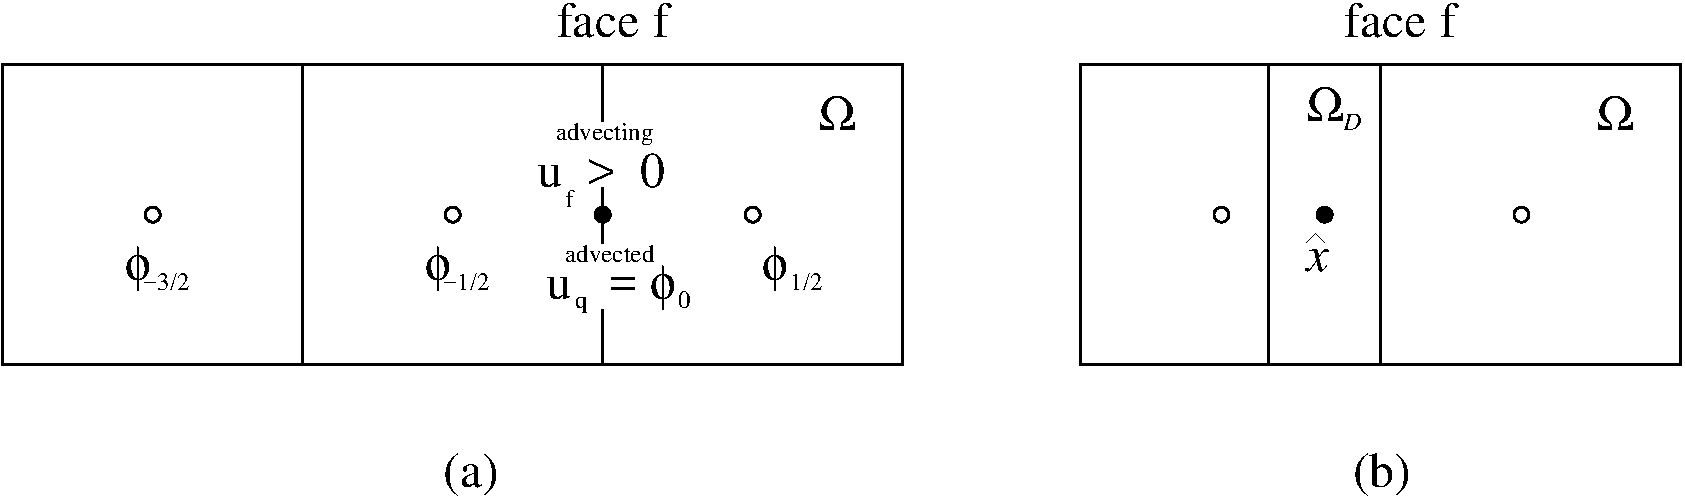
\includegraphics[width=\textwidth]{Figures/advect-ed-ing.pdf}
\end{center}
\caption{(a) The advected and advecting velocities in expression (\ref{advect-ed-ing-2}) 
  are both located on or near face $f$ (in this case $f=1-$). The reference control volume
$\Omega$ for the advected velocity component $u_q$ is also shown. The arrangement is the same
whatever the component $q$ but here the example of a horizontal advection ( case $f=1-$ ) is taken. 
The value of the advected velocity component $\bar u_q = \phi_0$ on the center of 
face $f$ (full disk) is interpolated (see text) from the values $\phi_{p}$ of $u_{q}$ on the nodes (open disks). 
(b) A more sophisticated interpolation predicts the value $\phi(\hat x)$ where $\hat x$ is
at the center of the ``donating'' region $\Omega_D$ (see text).}
\label{advect-ed-ing-fig}
\end{figure}
%\subsubsection{Momentum advection: tuned interpolations near the interface}
\label{tunedinter}

A slightly different estimate of the Superbee advected velocity is used near the interface. First we extend 
the definition of the interpolants as we shall predict $\bar u_q$ at a point $\hat x$ 
slightly upwind from $x_f$ using a new function $\hat f$ so that
\be
\phi_0 = \hat f(\hat x,\phi_{-3/2}, \phi_{-1/2}, \phi_{1/2},\phi_{3/2},{\rm sign}(u_f)). \label{mp}
\nd
We take  $\hat x = x_f - u_f \tau/2$ to be the midpoint of the fluxed region. (This is the region from which
flow lines crossing the face originate see Figure \ref{advect-ed-ing-fig}(b).)
The extended interpolant is defined for positive velocity %  $u_f>0$ 
as
\be
\hat f(\hat x,\phi_{-3/2}, \phi_{-1/2}, \phi_{1/2},\phi_{3/2},{\rm sign}(u_f)) = \phi_{-1/2} +  S |\hat x - x_{-1/2}|
\nd
and for negative velocity % $u_f<0$ 
as
\be
\hat f(\hat x,\phi_{-3/2}, \phi_{-1/2}, \phi_{1/2},\phi_{3/2},{\rm sign}(u_f)) = \phi_{1/2} -  S |\hat x - x_{1/2}|
\nd
The rationale behind this choice is as follows. For a time-independent advecting velocity field $u(\X,t)$, 
the integrals in expression
(\ref{barudef}) can be simplified
\be
\phi_0 = \bar u_q = \frac{\int_{\Omega_D}  u_f u_q \, {\rm d}\X}{ \int_{\Omega_D}  
u_f  \,{\rm d}\X}.  \label{barphi3}
\nd
where ${\Omega_D} $ is the ``donating region'' (see \cite{Tryggvason11})  from which
flow lines crossing the face originate. Then
since we approximate the advecting velocity $u_f$ by its midpoint value  the integral
can be further simplified as
\be 
\bar u_q = \frac 1{|\Omega_D|} \int_{\Omega_D}  u_q \, {\rm d}\X  \label{barphi4}
\nd
Since the ``midpoint'' at $\hat x$ is the center of mass of the donating region ${\Omega_D}$ 
the interpolation expression (\ref{mp}) follows. 

\subsubsection{VOF-consistent Momentum advection: staggered grids.}

In order to apply the above method on the staggered grid, 
the fluxes and control volumes of the momentum must be in
correspondence with the fluxes and control volumes of the VOF color
function.  This is realized by recreating in each velocity control
volume the necessary color fraction data. 

At the start of the velocity advection operations summarized by the operator 
$\LLL^h_{\rm conv}$ each velocity control volume say $\Omega_{i+1,j,k}$ overlaps two VOF control volumes
$\Omega_{i,j,k}$ and $\Omega_{i+1,j,k}$ ( see figure \ref{halffractions}) 
The following operations are performed:

\begin{enumerate}
\item Reconstruction of the volume fractions and density $C^{n}$ and $\rho^{n}$ in the staggered control volumes 
$\Omega_{i+1/2,j,k}$ corresponding to the momentum component $\rho u_1$, thus obtaining the ``half fractions'' $\tilde C^{n}$ and  $\tilde \rho^{n}$. 
\item Computation of the initial momentum component $\tilde g_1^{n} = \tilde \rho^{n} u_1^{n}$.
\item Split advection of the momentum in the $x$ direction 
using the method in the previous sections to obtain 
the first component of the new momentum $\hat g_1^{n+1}$.
\item Split advection in the $x$ direction of the volume fractions and density in the staggered control volumes 
using the volume of fluid method to obtain predicted densities $\hat\rho^{n+1,1}$.
\item Repeat the previous split advection operations for momentum and density in $y$ and $z$. At each time step, the sequence $x, y, z$
is permuted. Eventually one obtains $\hat g_1^{n+1}$ and $\hat\rho^{n+1}$.
\item Repeat the previous operations for the two other momentum components $g_2$ and  $g_3$. 
\item Extraction of the  new velocities components $\U^{*}=\hat \G^{n+1}/\hat\rho^{n+1}$.
\item In parallel, computation of $C^{n+1}$ from $C^n$ on the centered cells using
the VOF method. 

\end{enumerate}

We now cover the eight steps in detail. 
The reconstruction of the volume fractions in the staggered cells (step 1) implies considering each control volume for a velocity component, say $\Omega_1=\Omega_{i+1/2,j,k}$ for the $u_1$ component, and finding the ``half'' volume fraction
in each intersection $ \Omega_{i+1/2,j,k} \cap  \Omega_{i,j,k}$ and  $ \Omega_{i+1/2,j,k} \cap  \Omega_{i+1,j,k}$ 
(see Figure \ref{halffractions}). The ``half-fractions'' are found using the reconstruction parameters
$\alpha$, $\M$ in equation (\ref{mxalpha}) in the original
centered control volume, and then computing the corresponding volume fractions in the half 
cells. Addition of the two half fractions leads to an estimate of the volume fraction $\tilde C^n_{i+1/2,j,k}$ in the staggered cells, and thus of the densities $\tilde \rho^n_{i+1/2,j,k}$. 

In step 2, now that the staggered cell densities at the beginning of the time step are known, 
obtain the momentum component $g^n_{1,i+1/2,j,k} = \rho^{n}_{i+1/2,j,k} u^{n}_{1,i+1/2,j,k}$. 
This momentum component can be advected (step 3) using the method described in the previous section, to 
obtain  $\hat g^{n+1}_{1,i+1/2,j,k}$  in a  conservative manner
following equation (\ref{advect-ed-ing}). 
Similarly the  volume fractions in the staggered cells are also reconstructed and advected in
direction $x_1$  in step 4. 
Then in step 5 the other directionally split advections are performed. 
After each direction, the newly obtained densities and advected velocities are used for the next direction
but the advecting velocities remain the same. The central velocity stepping is discussed 
below equation (\ref{tildeudef}) above. 
Finally the advections are performed in each of the three systems of staggered cells (step 6) to obtain  
$\hat C^{n+1}_{i+1/2,j,k} = \hat C^{n,4}_{i+1/2,j,k}$  where the 
notation $C^{n,m}$ was introduced in equation (\ref{sumf2}) and $m$ indicates which direction of the 
split time step was performed. Then $\hat \rho^{n+1}_{i+1/2,j,k} = \rho_1 \hat  C_{i+1/2,j,k} + \rho_2 ( 1 - \hat C_{i+1/2,j,k} ) $ obtains.
Finally the $\LLL_{\rm conv}$ operator is obtained as (step 7) 
\be
 \LLL_{\rm conv} =  \frac 1 \tau (\hat \G^{n+1} - \tilde \rho^{n} \U^n \label{unp11})
\nd
where as above we use the $\tilde \rho$ notation to indicate that the density has been 
reconstructed in the staggered cells.
In the absence of the other operators in $\LLL_2$ this would result 
in
\be
\U^* = \hat \G^{n+1}/ \hat \rho^{n+1}.
\nd
However (leaving aside the pressure and other contributions in equation  (\ref{fotm}))
 the momentum on the staggered cells at the beginning of the next
time step is not equal to the momentum $\hat \rho^{n+1} \U^{n+1}$ at the end of the previous 
time step but is rather defined as $\tilde \rho^{n+1} \U^{n+1}$ where  $\tilde \rho^{n+1}$ is 
obtained at beginning of the time step from the half-fractions. That is, $C^{n+1}$ is computed 
directly from $C^{n}$ on the centered cells (step 8) and this allows to find 
 $\tilde C^{n+1}$ and from it, $\tilde \rho^{n+1}$ , by running again step 1. These densities  $\tilde \rho^{n+1}$ are not
the same as the  $\hat \rho^{n+1}$  densities of the previous time step. This implies non conservation of the momentum.
We note that  attempting to always use only the three sets
 $C^{n}_{i+1/2,j,k}$,  $C^{n}_{i,j+1/2,k}$,  $C^{n}_{i,j,k+1/2}$ and evolve them by 
the VOF method on the staggered cells 
would maintain conservation but result in the three staggered grids evolving independently of each other and
eventually diverging.
\begin{figure}
\begin{center}
    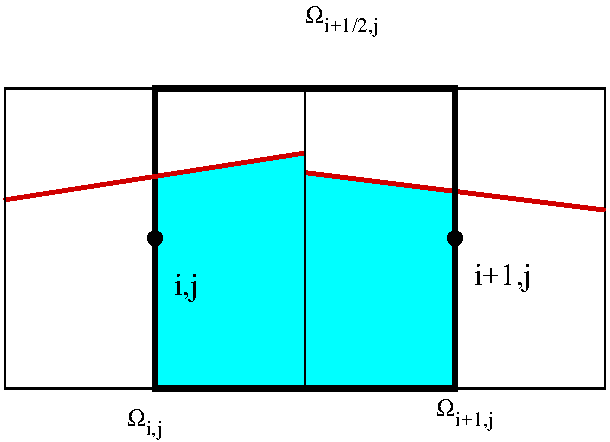
\includegraphics[width=0.5\textwidth]{Figures/halffractions.pdf}
\end{center}
\caption{Computation of the staggered fractions from the half-fractions}
\label{halffractions}
\end{figure}
\clearpage

\subsection{Description of the other time-split terms}

The other time-split terms in equation (\ref{conspredictedvel}) and in the projection
step (\ref{fotm}) are solved in a standard centered way. The density on the faces
of the central cells $\Omega_{i,j,k}$ is estimated using a centered average
$\rho_{i+1/2,j,k} = (\rho_{i+1/2,j,k} + \rho_{i+1/2,j,k})/2$. Although this is less accurate and consistent
than the usage of the half fractions $\hat \rho_{i+1/2,j,k}$ described above the average 
is used in these terms both for simplicity reasons and because tests have shown the usage
of $\hat \rho_{i+1/2,j,k}$ to lead to less stable simulations than the centered average. 

The velocities in the diffusion term are introduced in an explicit way. Although this requires small
time steps of the order $\rho h^2/\mu$ the capillary restriction on time steps
is usually even smaller, being of order $\tau = (\rho h^3/\sigma)^{1/2}$. The two restrictions
become of the same order when $h \sim l_{\mu \sigma}$ where $l_{\mu \sigma} = \mu^2 / (\sigma \rho)$ 
is the length at which the viscous and capillary terms balance. For water, this length is 
of the order of 10 nanometers, and grids of that size are not used in the flows we consider. 
However, should the velocities be treated in an implicit manner, we do not believe this would
change the conclusions of this paper. 

Surface tension is computed using the Continuous Surface Force method proposed by 
\cite{brackbill92}, together with an estimate of the curvature through the computation
of height functions, in a manner that closely follows the method of \cite{popinet09}. 
The external forces in equation (\ref{conspredictedvel}) 
are only gravity and are computed in a trivial manner with 
$\frac 1 {\rho^{n+1}} \LLL_{ext} =  \G$, where gravity $\G$  is a constant. 


